\documentclass[11pt,a4paper]{article}
% Preamble for levy_reset_extremes.tex (loaded after \documentclass).
\usepackage[T1]{fontenc}
\usepackage[utf8]{inputenc}
\usepackage{lmodern}
\usepackage{amsmath,amssymb,amsthm,mathtools}
\usepackage[margin=26mm]{geometry}
\usepackage{microtype}
\usepackage{booktabs,array}
\usepackage{graphicx}
\usepackage{caption}
\usepackage[dvipsnames]{xcolor}
\usepackage{fancyhdr}
\usepackage{xurl}
\usepackage[colorlinks=true,linkcolor=black,citecolor=black,urlcolor=MidnightBlue]{hyperref}
\captionsetup{font=small,labelfont=bf}
\pagestyle{fancy}
\fancyhf{}
\fancyhead[L]{\small Spectrally negative L\'evy resetting extremes}
\fancyhead[R]{\small Research manuscript}
\fancyfoot[C]{\thepage}
\setlength{\headheight}{14pt}
\setlength{\emergencystretch}{3em}
\setlength{\parskip}{0.4em}
\renewcommand{\arraystretch}{1.18}
\numberwithin{equation}{section}
\theoremstyle{plain}
\newtheorem{theorem}{Theorem}[section]
\newtheorem{proposition}[theorem]{Proposition}
\newtheorem{lemma}[theorem]{Lemma}
\newtheorem{corollary}[theorem]{Corollary}
\theoremstyle{remark}
\newtheorem{remark}[theorem]{Remark}
\newcommand{\PP}{\mathbb P}
\newcommand{\EE}{\mathbb E}
\newcommand{\R}{\mathbb R}
\newcommand{\var}{\mathrm{var}}
\newcommand{\dd}{\,\mathrm d}


\title{Fixed-horizon extremes of spectrally negative L\'evy processes with Poisson resetting\\[4pt]
\large The endpoint after a high peak, and the constant in Remark~3 of D\k{e}bicki, Hashorva and Michna}
\author{Anonymous}
\date{27 October 2026. Version 1.0.0-candidate; first version 20 October 2026.\\ DOI \href{https://doi.org/10.5281/zenodo.23689354}{10.5281/zenodo.23689354}}

\begin{document}
\maketitle
\thispagestyle{fancy}

\noindent\textbf{Research manuscript. Not externally refereed.}

\begin{abstract}
\noindent
A process that wanders randomly but is sent back to a home position at random times is a basic model in search, foraging, queueing with catastrophes and risk theory. We take such a process to be a spectrally negative L\'evy process, that is, one with no upward jumps, with resets at the times of a Poisson clock, and we start it in its long-run state. We then ask where it is at the end of a fixed time window, given that its maximum over the window was very high. Up to an error smaller than any exponential order, there are only two answers: either no reset has happened and the process ends close to its peak, or a reset has happened and it ends at an ordinary level. We give the odds of the two answers, the full endpoint law in each case, and a construction of the whole conditional path, in which the height of the peak above the threshold is exponentially distributed and independent of everything else. The leading constants come from a standard first-cycle computation. What is new is an explicit error bound in total variation that holds uniformly over all endpoint sets, together with the conditional path law and its fixed-threshold versions. For Brownian motion the result supplies the constant left unspecified in Remark~3 of D\k{e}bicki, Hashorva and Michna (2026) and shows that their two bounds on it are strict. We also extend the theorem to random reset positions, and check every formula against an exact-sampling simulation of the original process.
\end{abstract}

\section{Introduction}\label{sec:intro}

\paragraph{Why resetting and maxima.}
Resetting a random motion to a fixed point at random times was introduced to physics as a search strategy: a diffusing searcher that returns home at rate $\lambda$ finds a target faster on average than one that never returns \cite{EM2011,EMS2020}. The same picture describes an animal that forages from a nest or den \cite{PKR2020}, a queue that is emptied by catastrophes \cite{DGNR2003}, a Markov process that is restarted \cite{APZ2013}, and a randomised algorithm that is restarted when it runs too long \cite{LSZ1993}. In ruin theory the surplus of an insurer is a L\'evy process with downward jumps (the claims) \cite{AA2010,Kyp2014}, and a reset is a recapitalisation or regulatory intervention that restores the reserve to a target level. In finance the joint law of a running maximum and a terminal value is exactly what is needed to price lookback and barrier payoffs \cite{GSG1979}; we do not suggest that resetting models are good price models, only that this joint law is the natural object.

In all of these settings one asks about extremes: how far did the searcher, animal or surplus go during a window of length $T$, and what does a far excursion imply about the state at the end of the window? Extreme-value statistics of strongly correlated processes are surveyed in \cite{MPS2020}. For resetting processes, records and maxima have been studied with renewal methods \cite{SP2021,MMSS2022}, as has the time of the maximum \cite{MMS2021}. Resetting at a time-dependent rate, which we do not treat, is studied in \cite{PKE2016}.

\paragraph{The result in one sentence.}
\emph{Given that the process had an extreme peak during the window, it either ends near that peak, because no reset has happened yet, or it has been reset and ends at an ordinary level. The odds of the two cases converge to explicit constants, about $53:47$ in the standard Brownian example, and the amount by which the peak exceeds the threshold is memoryless, exponential with mean $1/\beta$.}

Figure~\ref{fig:main}(a) shows the two kinds of path. In formulas (Theorem~\ref{thm:endpoint}), with $H_T$ the maximum over $[0,T]$, $Y_T$ the endpoint and $r$ the reset position,
\begin{equation}\label{eq:informal}
 \PP(H_T>u,\ Y_T\in B)\;\approx\;e^{-\beta(u-r)}\big[\,Q_T(B-u)\;+\;K_T(B)\,\big],
\end{equation}
where $Q_T$, shifted up by $u$, describes paths with no reset, and $K_T$, which does not move with $u$, describes paths that were reset after the peak. The error is bounded explicitly, uniformly over all sets $B$, including sets that move with $u$.

\begin{figure}[t]
\centering
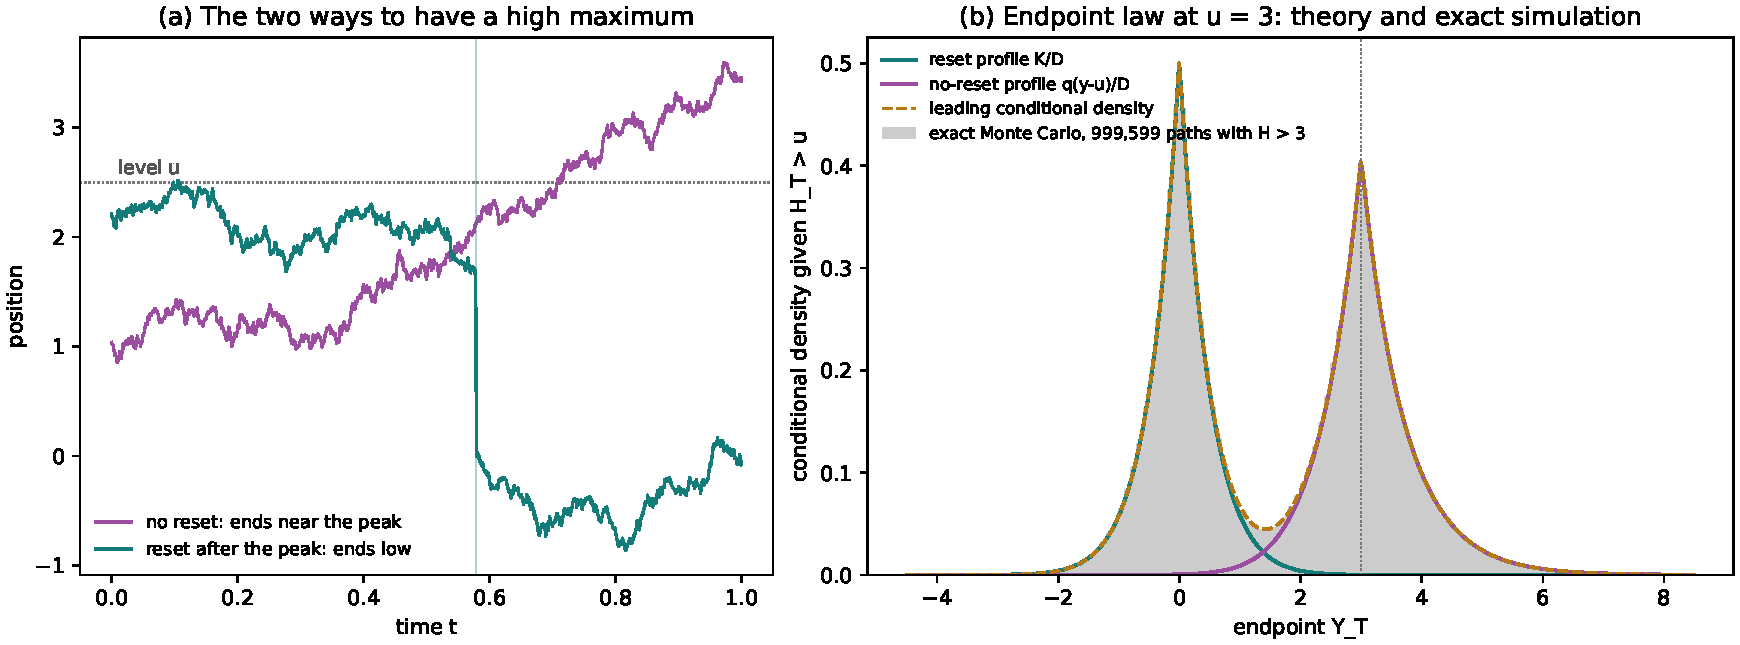
\includegraphics[width=\textwidth]{figures/resetting_endpoint_profiles.pdf}
\caption{Zero-drift Brownian motion with reset rate, variance and horizon equal to one, reset to $r=0$, started in stationarity. \textbf{(a)} Two simulated paths whose maximum exceeds $u=2.5$ (shown on a time grid of step $10^{-3}$, for illustration only): one is not reset and ends near its peak; the other is reset after its peak (vertical line) and ends at an ordinary level. \textbf{(b)} The conditional law of the endpoint $Y_T$ given $H_T>3$. The grey histogram comes from the exact-sampling Monte Carlo of Section~\ref{sec:numerics} (bin width $0.1$, no time discretisation); the curves are the leading-order profiles of Theorem~\ref{thm:endpoint}, namely $K_T(\mathrm dy)/(D_T\,\mathrm dy)$ (reset, centred at $r=0$) and $q_T(y-u)/D_T$ (no reset, centred at $u=3$). Because the no-reset profile is a translate, the two humps are $u$ apart for every $u$; their masses tend to $1-A(T)/D_T\approx0.469$ and $A(T)/D_T\approx0.531$.}
\label{fig:main}
\end{figure}

\paragraph{The source question.}
D\k{e}bicki, Hashorva and Michna \cite{DHM2026} studied stationary Brownian motion with exponential resetting. They found the tail of the maximum (their Theorem~5) and the joint tail with a terminal threshold proportional to $u$ (their Theorem~6). In their Remark~3 they conjectured that, for the terminal threshold $0$, which Theorem~6 does not cover,
\begin{equation}\label{eq:conj}
 \PP\Big(\sup_{0\le t\le T}Y_t>u,\ Y_T>0\Big)\sim C_T\,e^{-\alpha u},\qquad u\to\infty,
\end{equation}
with $e^{\alpha x_R}\Phi(\alpha\sqrt T)\le C_T\le e^{\alpha x_R}\big[\Phi(\alpha\sqrt T)+\lambda\int_0^T\Phi(\alpha\sqrt s)\dd s\big]$. Their setting is: unit variance; drift written as $W_t-ct$; reset rate $\lambda$ to position $x_R$; stationary initialisation; supremum over $[0,T]$; strict event inequalities ($H_T>u$, $Y_T>0$); and $\alpha=\sqrt{2\lambda}$. Their bounds on $C_T$ are stated with ``$\le$''. Corollary~\ref{cor:brownian} of the present paper identifies $C_T$ and proves that both bounds are in fact strict; that strictness is a result of this paper, not a statement of \cite{DHM2026}. In the notation of this paper $\alpha$ is the rate $\beta$ at $\sigma=1$ (it is the same number, not a correction), $x_R=r$ and $c=-\mu$. We avoid the letter $\alpha$ for the rate because it usually denotes a stability index in the L\'evy-flight literature.

\paragraph{What is standard and what is new.}
We want to be precise about credit. The leading constant in \eqref{eq:informal}, and hence $C_T$, comes from a standard first-cycle (renewal) computation of the kind D\k{e}bicki et al.\ use for their own Theorem~5, combined with the classical Wiener--Hopf fact that the stationary law has an exactly exponential right tail. Once the conjecture is set up this way, computing $C_T$ is not difficult; we \emph{supply} the constant and prove that the bounds are strict, rather than claiming a hard resolution. The new contributions are:
\begin{enumerate}
\item an explicit error bound for \eqref{eq:informal} in total variation, uniform over all endpoint sets and in particular over sets that depend on $u$ (Theorem~\ref{thm:endpoint}); a naive renewal argument gives the leading term for each fixed set but not this uniformity (Remark~\ref{rem:naive});
\item the conditional law of the whole marked path given a high maximum, with the same error rate (Theorem~\ref{thm:path}), and quantitative statements for the overshoot, the first reset time and fixed terminal thresholds (Propositions~\ref{prop:marks}--\ref{prop:pathlimit});
\item exactness above an explicit threshold for bounded-variation inputs (Corollary~\ref{cor:bv}), and an extension to random reset positions (Theorem~\ref{thm:random}).
\end{enumerate}
Table~\ref{tab:prior} compares these statements with the closest earlier results.

\begin{table}[h]
\centering\small
\setlength{\tabcolsep}{3pt}\begin{tabular}{@{}>{\raggedright\arraybackslash}p{2.8cm}>{\raggedright\arraybackslash}p{1.7cm}>{\raggedright\arraybackslash}p{1.2cm}>{\raggedright\arraybackslash}p{3.3cm}>{\raggedright\arraybackslash}p{3.0cm}>{\raggedright\arraybackslash}p{1.0cm}@{}}
\toprule
Work & Start & Horizon & Observable & Type of result & Path law \\
\midrule
Singh--Pal \cite{SP2021} & at reset point & fixed & max, time of max & exact renewal formula & no\\
Mori et al.\ \cite{MMS2021} & stationary & fixed & time of max & distributional & no\\
D\k{e}bicki et al.\ \cite{DHM2026} & stationary & fixed & max; max with $Y_T>zu$ & scalar asymptotics & no\\
This paper & stationary & fixed & max and endpoint, all sets & total variation, explicit error & yes\\
\bottomrule
\end{tabular}
\caption{Closest earlier results for Brownian or L\'evy resetting extremes. We are not aware of an earlier result giving this uniform endpoint-measure expansion for general spectrally negative L\'evy input.}
\label{tab:prior}
\end{table}

\paragraph{Why no upward jumps.}
The argument needs two facts. First, the stationary law has an \emph{exactly} exponential right tail, with an exponential continuation that dominates its density everywhere \eqref{eq:pi}. Second, a high excursion is, up to a negligible error, made in the cycle that is running at time $0$, because a freshly reset cycle has a much lighter fixed-horizon tail \eqref{eq:doob}. Spectral negativity gives both. A process that cannot jump upwards must pass every level continuously, so its ladder heights, and hence the stationary tail, are exactly exponential, and the overshoot of the peak is memoryless. With upward jumps both facts fail. If the upward jumps are light-tailed (a Cram\'er-type condition), the stationary tail is exponential only asymptotically, the density has no exact exponential continuation, and the overshoot follows a ladder-overshoot law rather than $\mathrm{Exp}(\beta)$. If the upward jumps are heavy-tailed, as for two-sided stable L\'evy flights, there is no $\beta$ at all: the stationary tail is polynomial, a single big jump can produce the peak in \emph{any} cycle, and the first-cycle principle behind \eqref{eq:later} breaks down. That regime, which includes the L\'evy-flight resetting models of \cite{KMSS2014,MMSS2022,ZP2026}, needs a different analysis.

\paragraph{Roadmap.}
Section~\ref{sec:model} sets up the model and gives a plain-language glossary. Section~\ref{sec:thm1} states and proves the endpoint theorem. Section~\ref{sec:thresholds} turns it into statements about terminal thresholds. Section~\ref{sec:paths} describes the conditional path, the first reset and the overshoot. Section~\ref{sec:brownian} makes everything explicit for Brownian motion, gives the constant $C_T$, and discusses when the asymptotic regime begins. Section~\ref{sec:bv} proves exactness for bounded-variation inputs and extends the theorem to random reset positions. Section~\ref{sec:numerics} reports analytic and Monte Carlo checks, and Section~\ref{sec:scope} lists open problems.

\section{Model, notation and a glossary}\label{sec:model}

Let $\xi=(\xi_t)_{t\ge0}$ be a spectrally negative L\'evy process with $\xi_0=0$, that is, a L\'evy process with no positive jumps, and assume that its paths are not almost surely nonincreasing. Deterministic positive drift is allowed. Because there are no upward jumps, all positive exponential moments exist, and we write
\[
 \psi(\theta)=\log\EE e^{\theta\xi_1}\ (\theta\ge0),\qquad M_t=\sup_{0\le s\le t}\xi_s .
\]
The function $\psi$ is finite and strictly convex on $[0,\infty)$, with $\psi(\theta)\to\infty$, so for $\lambda>0$ the equation $\psi(\beta)=\lambda$ has a unique positive root $\beta$, at which $\psi'(\beta)>0$. Put
\begin{equation}\label{eq:a}
 a=\frac{\lambda}{\beta\psi'(\beta)} .
\end{equation}

Let $N$ be an independent Poisson process of rate $\lambda$ and fix $r\in\R$. Between the jumps of $N$ the process moves by independent L\'evy increments, and at each jump it is set to $r$:
\begin{equation}\label{eq:sde}
 Y_t=Y_0+\xi_t+\int_{(0,t]}(r-Y_{s-})\dd N_s .
\end{equation}
We start $Y$ in its invariant law, which is the law of $r+\xi_{e_\lambda}$ with $e_\lambda$ an independent $\mathrm{Exp}(\lambda)$ time. To see this, look back from time $0$: the age of the current cycle is $\mathrm{Exp}(\lambda)$, and during that age the process has moved by free L\'evy increments from $r$. The invariant law is unique, because two copies driven by the same clock and the same increments coincide after the first reset, which happens almost surely.

We write $X$ for the reset process freshly started at $r$, and $\PP_r(X_t\in\cdot)$ for its law at time $t$. Fix $T>0$ and put
\[
 H_T=\sup_{0\le t\le T}Y_t,\qquad \tau=\inf\{t>0:N_t>0\},\qquad b=u-r .
\]
The Esscher law $\PP^{(\beta)}$ on free L\'evy paths is defined by
\begin{equation}\label{eq:esscher}
 \frac{\mathrm d\PP^{(\beta)}}{\mathrm d\PP}\bigg|_{\mathcal F_t}=e^{\beta\xi_t-\lambda t}.
\end{equation}
For a finite signed measure we use the full variation norm $\|\eta\|_\var=|\eta|(\Omega)$. For two probability laws this is twice $\sup_B|P(B)-Q(B)|$, so a reader who prefers the supremum convention can halve every bound below.

The central quantities are
\begin{equation}\label{eq:AD}
 A(t)=a\,e^{-\lambda t}\EE e^{\beta M_t},\qquad D_T=A(T)+\lambda\int_0^TA(s)\dd s,
\end{equation}
which are finite by \eqref{eq:doob} below, together with two finite measures on $\R$:
\begin{equation}\label{eq:K}
 K_T(B)=\lambda\int_0^TA(s)\,\PP_r(X_{T-s}\in B)\dd s,
\end{equation}
and $Q_T(\mathrm dw)=q_T(w)\dd w$ with
\begin{equation}\label{eq:q}
 q_T(w)=a\beta e^{-\beta w}\,\PP^{(\beta)}(M_T-\xi_T>-w).
\end{equation}
For $w>0$ the probability in \eqref{eq:q} equals one. By time reversal of L\'evy processes, $M_T-\xi_T$ has the law of $\sup_{s\le T}(-\xi_s)$ under $\PP^{(\beta)}$, so \eqref{eq:q} needs no transition density.

\begin{table}[h]
\centering\small
\begin{tabular}{@{}ll@{}}
\toprule
Symbol & Meaning in words\\
\midrule
$\beta$ & decay rate of the stationary right tail; the overshoot of a high peak is $\mathrm{Exp}(\beta)$, mean $1/\beta$\\
$a$ & stationary tail constant: $\PP(Y>r+x)=a\,e^{-\beta x}$ for every $x\ge0$\\
$A(t)$ & weight of a high peak made in an initial cycle that survives at least $t$ time units\\
$D_T$ & total weight of a high peak in the window: $\PP(H_T>u)\approx D_T\,e^{-\beta(u-r)}$\\
$Q_T$ & endpoint law, measured from $u$, of high-peak paths with no reset (mass $A(T)$)\\
$K_T$ & endpoint law of high-peak paths that were reset after the peak (mass $D_T-A(T)$)\\
\bottomrule
\end{tabular}
\caption{Glossary. The odds of ``no reset'' against ``reset'' given a high peak are $A(T):(D_T-A(T))$.}
\label{tab:glossary}
\end{table}

\begin{remark}[Stable inputs]\label{rem:stable}
For a spectrally negative $\alpha$-stable input with $\psi(\theta)=\theta^\alpha$, $1<\alpha\le2$, we get $\beta=\lambda^{1/\alpha}$ and $a=1/\alpha$, so the tail constant does not depend on $\lambda$. The case $\alpha=2$ is Brownian motion with $\sigma^2=2$. For $\alpha<1$ the spectrally negative stable process is nonincreasing and is excluded, but with an added positive drift it falls under Corollary~\ref{cor:bv}.
\end{remark}

\section{The endpoint theorem}\label{sec:thm1}

\begin{theorem}\label{thm:endpoint}
Under the assumptions of Section~\ref{sec:model}, $Q_T(\R)=A(T)$ and $K_T(\R)=D_T-A(T)$. For every $u>r$, with $b=u-r$, and every $\gamma>\beta$,
\begin{equation}\label{eq:main}
 \Big\|\PP(H_T>u,\ Y_T\in\cdot)-e^{-\beta b}\big\{Q_T(\cdot-u)+K_T(\cdot)\big\}\Big\|_\var
 \le R_\gamma(b,T):=\Big(\frac{a\beta}{\gamma-\beta}+\lambda T\Big)e^{T\psi(\gamma)-\gamma b}.
\end{equation}
Here $Q_T(\cdot-u)$ is the image of $Q_T$ under $w\mapsto u+w$. The bound holds uniformly over all Borel endpoint sets, including sets that depend on $u$, and it also holds before the path is projected to its endpoint (see \eqref{eq:pathlevel}). In particular $|\PP(H_T>u)-D_Te^{-\beta b}|\le R_\gamma(b,T)$.
\end{theorem}

Since $\psi$ is finite on all of $[0,\infty)$, we may take $\gamma$ as large as we like. For fixed $T$ the error is therefore $o(e^{-\eta b})$ for every $\eta>0$, which is much smaller than the leading term $e^{-\beta b}$. This would fail if positive jumps were allowed, since then $\psi$ can be infinite. The constants depend on $\gamma$ and $T$, and nothing is claimed uniformly over growing horizons; Section~\ref{sec:onset} discusses how large $b$ must be in practice.

\subsection{The stationary density and its exponential continuation}

\begin{lemma}\label{lem:pi}
Let $\pi$ be the density of $Y_0-r$. Then $\EE e^{\beta I}=a$, where $I\le0$ has the law of the infimum of $\xi$ up to $e_\lambda$, and
\begin{equation}\label{eq:pi}
 \pi(x)=a\beta e^{-\beta x}\ (x\ge0),\qquad 0\le\pi(x)\le a\beta e^{-\beta x}\ (x\in\R),
\end{equation}
for almost every $x$. In particular $0<a\le1$ and $\PP(Y_0>r+x)=a e^{-\beta x}$ for $x\ge0$.
\end{lemma}

\begin{proof}
The Wiener--Hopf factorisation at an independent exponential time \cite[Section~2.1]{KKR2012} gives independent random variables $E_\beta\sim\mathrm{Exp}(\beta)$ and $I\le0$, distributed respectively as the supremum and the infimum of $\xi$ up to $e_\lambda$, such that $\xi_{e_\lambda}\overset d=E_\beta+I$. (The supremum and infimum of the same path are in general dependent; only the two factors are independent.) (Pure positive drift has $I=0$.) Convolution gives, for almost every $x$,
\[
 \pi(x)=\beta e^{-\beta x}\,\EE\big[e^{\beta I}\mathbf 1_{\{I<x\}}\big].
\]
The strict and non-strict indicators differ only at atoms of $I$, which form a Lebesgue-null set, so the choice does not matter for a density. For $0\le\theta<\beta$, taking moment generating functions gives $\EE e^{\theta I}=\frac{\lambda}{\lambda-\psi(\theta)}\cdot\frac{\beta-\theta}{\beta}$. As $\theta\uparrow\beta$ the left side converges to $\EE e^{\beta I}$ by dominated convergence (since $0\le e^{\theta I}\le1$), and the right side converges to $\lambda/(\beta\psi'(\beta))=a$. For $x\ge0$ the indicator equals one, which gives the equality in \eqref{eq:pi}; for $x<0$ it is at most one, which gives the inequality.
\end{proof}

The same conclusion follows from the resolvent formula $\pi(x)=\lambda\big(e^{-\beta x}/\psi'(\beta)-W^{(\lambda)}(-x)\big)$ of \cite[Theorem~2.7(iv)]{KKR2012}, but we need only \eqref{eq:pi}.

\begin{lemma}\label{lem:doob}
For $\gamma>\beta$, every $t\ge0$ and every real $z$,
\begin{equation}\label{eq:doob}
 \PP(M_t>z)\le e^{t\psi(\gamma)-\gamma z}.
\end{equation}
In particular $\EE e^{\beta M_t}<\infty$.
\end{lemma}

\begin{proof}
For $z\le0$ the right side is at least one, because $\psi(\gamma)>\psi(\beta)=\lambda>0$. For $z>0$, the process $e^{\gamma\xi_s}$ is a nonnegative submartingale, because $\psi(\gamma)\ge0$. Doob's maximal inequality gives $\PP(\sup_{s\le t}e^{\gamma\xi_s}\ge e^{\gamma z})\le e^{-\gamma z}\EE e^{\gamma\xi_t}=e^{t\psi(\gamma)-\gamma z}$. Integrating the tail bound against $\beta e^{\beta z}$ gives the finiteness of $\EE e^{\beta M_t}$.
\end{proof}

\subsection{Proof of Theorem~\ref{thm:endpoint}}

\emph{Strategy.} Up to a negligible error, the only way to reach a high maximum is to start high in the cycle that is running at time $0$. We replace the true starting density by its pure exponential continuation, which makes every quantity explicit, and we bound the two errors this introduces: exceedances in later cycles, which we drop, \eqref{eq:later}; and extra starting mass below $r$, which we add, \eqref{eq:cont}.

\paragraph{The probability space.}
We build $Y$ from independent ingredients: the initial offset $x=Y_0-r$ with density $\pi$; the free L\'evy path $\xi^{(0)}$ that drives the initial cycle; the reset clock $N$; and a sequence of independent free L\'evy paths $\xi^{(1)},\xi^{(2)},\dots$ that drive the cycles started at the reset epochs $\sigma_1<\sigma_2<\cdots$. Write $\Theta$ for everything except $x$. The path $Y_{[0,T]}$, the first-reset mark $\widehat\tau$ ($=\tau$ if $\tau\le T$ and $=\dagger$ otherwise) and every other quantity below are measurable functions of $(x,\Theta)$, which takes values in a Polish product space $\R\times\mathsf E_\Theta$. All measures below live on this space. On $\{\tau=s\le T\}$ the initial-cycle maximum is $r+x+\sup_{v<s}\xi^{(0)}_v$. Because an independent exponential time is almost surely not a jump time of $\xi^{(0)}$, this equals $r+x+M^{(0)}_s$ almost surely. Let
\[
 E_u=\big\{x+M^{(0)}_{\tau\wedge T}>b\big\}
\]
be the event that the initial cycle exceeds $u$ before its first reset, or before $T$ if there is none.

\paragraph{Three measures.}
Define $\mu_u=\PP\big((x,\Theta)\in\cdot\,,\ H_T>u\big)$, which is the object of interest. Let $\nu(\mathrm dx)=a\beta e^{-\beta x}\dd x$ on $\R$ (a $\sigma$-finite measure), and set
\[
 \mathsf V_u=\big(\nu\otimes\PP_\Theta\big)\big|_{E_u},\qquad
 \mathsf C_u=\big((\nu-\pi)\otimes\PP_\Theta\big)\big|_{E_u},\qquad
 \mathsf L_u=\PP\big((x,\Theta)\in\cdot\,,\ H_T>u,\ E_u^c\big).
\]
By Lemma~\ref{lem:pi}, $\nu-\pi\ge0$, so $\mathsf C_u\ge0$; also $\mathsf L_u\ge0$. Since $E_u\subset\{H_T>u\}$, the measure $\mu_u$ is the sum of $(\pi\otimes\PP_\Theta)|_{E_u}=\mathsf V_u-\mathsf C_u$ and $\mathsf L_u$. Hence
\begin{equation}\label{eq:pathlevel}
 \mu_u-\mathsf V_u=\mathsf L_u-\mathsf C_u,\qquad \|\mu_u-\mathsf V_u\|_\var\le\mathsf L_u(\Omega)+\mathsf C_u(\Omega).
\end{equation}
Total variation can only decrease under a measurable map, so it is enough to bound the two masses and then to identify the endpoint image of $\mathsf V_u$.

\paragraph{Later cycles (expanding the bound \eqref{eq:later}).}
On $\{H_T>u\}\cap E_u^c$ some cycle started at a reset epoch $\sigma_k\le T$ exceeds $u$. That cycle starts at $r$ and runs for a time $\ell_k\le T-\sigma_k\le T$, so its maximum is at most $r+\sup_{v\le T}\xi^{(k)}_v$. The path $\xi^{(k)}$ is independent of the clock $N$, and hence of $\sigma_k$ and of whether $\sigma_k\le T$. This is exactly the strong Markov property of the reset process at its reset epochs. A union bound over $k$ therefore gives
\begin{equation}\label{eq:later}
 \mathsf L_u(\Omega)\le\sum_{k\ge1}\PP(\sigma_k\le T)\,\PP(M_T>b)=\EE N_T\,\PP(M_T>b)=\lambda T\,\PP(M_T>b)\le\lambda T\,e^{T\psi(\gamma)-\gamma b},
\end{equation}
using \eqref{eq:doob}. Because $r<u$, a reset itself cannot cause an exceedance.

\paragraph{Continuation error (expanding the bound \eqref{eq:cont}).}
The measures $\nu$ and $\pi$ agree on $[0,\infty)$, so $\mathsf C_u$ charges only $x<0$. The restriction $E_u$ uses the reset clock through $\tau\wedge T$. The event $\{x+M^{(0)}_{\tau\wedge T}>b\}$ is contained in $\{x+M^{(0)}_T>b\}$, so we may drop the clock, whose weight is at most one. With $\nu-\pi\le\nu$ and \eqref{eq:doob},
\begin{equation}\label{eq:cont}
 \mathsf C_u(\Omega)\le\int_{-\infty}^0a\beta e^{-\beta x}\,\PP(M_T>b-x)\dd x
 \le a\beta\,e^{T\psi(\gamma)-\gamma b}\int_{-\infty}^0e^{(\gamma-\beta)x}\dd x=\frac{a\beta}{\gamma-\beta}\,e^{T\psi(\gamma)-\gamma b}.
\end{equation}
Adding \eqref{eq:later} and \eqref{eq:cont} gives the bound $R_\gamma(b,T)$ for $\|\mu_u-\mathsf V_u\|_\var$.

\paragraph{Evaluation after a reset.}
Condition on $\tau=s\in(0,T)$ and on $\xi^{(0)}$ up to $s$. Then $E_u$ is the event $x>b-M^{(0)}_s$, and $\nu\big((b-M^{(0)}_s,\infty)\big)=a\,e^{-\beta b}e^{\beta M^{(0)}_s}$. Multiplying by the clock density $\lambda e^{-\lambda s}$ and averaging over the free path gives the weight
\begin{equation}\label{eq:resetweight}
 e^{-\beta b}\,\lambda A(s)\dd s .
\end{equation}
After the reset at $s$ the process is a fresh copy of $X$ started at $r$, independent of everything before, so its endpoint has law $\PP_r(X_{T-s}\in\cdot)$. Integrating over $s$ shows that this part of the endpoint image of $\mathsf V_u$ is $e^{-\beta b}K_T$.

\paragraph{Evaluation without a reset.}
On $\{\tau>T\}$ change variables from $x$ to $w=Y_T-u=x+\xi^{(0)}_T-b$. The restriction $x>b-M^{(0)}_T$ becomes $M^{(0)}_T-\xi^{(0)}_T>-w$, and the endpoint density of $\mathsf V_u$ at $u+w$ is
\[
 a\beta e^{-\beta b}e^{-\beta w}\,e^{-\lambda T}\EE\big[e^{\beta\xi_T}\mathbf 1_{\{M_T-\xi_T>-w\}}\big]=e^{-\beta b}q_T(w),
\]
by \eqref{eq:esscher}. Before the change of variables the same mass is $e^{-\lambda T}\EE[a e^{-\beta b}e^{\beta M_T}]=e^{-\beta b}A(T)$. This proves $Q_T(\R)=A(T)$, and \eqref{eq:resetweight} gives $K_T(\R)=\lambda\int_0^TA=D_T-A(T)$. The endpoint image of $\mathsf V_u$ is therefore $e^{-\beta b}\{Q_T(\cdot-u)+K_T\}$, and \eqref{eq:main} follows. Taking total masses gives the bound for $\PP(H_T>u)$. \qed

\begin{remark}[A sharper remainder]\label{rem:sharp}
Two cruder steps can be refined at no cost. Write $q=\psi(\gamma)$. In \eqref{eq:later}, Campbell's formula for the reset epochs gives $\mathsf L_u(\Omega)\le\lambda\int_0^T\PP(M_{T-s}>b)\dd s\le\lambda e^{-\gamma b}(e^{qT}-1)/q$. In \eqref{eq:cont}, keeping the initial-cycle length $\tau\wedge T$ gives the factor $\EE e^{q(\tau\wedge T)}=e^{(q-\lambda)T}+\lambda\big(e^{(q-\lambda)T}-1\big)/(q-\lambda)$ in place of $e^{qT}$ (read as $1+\lambda T$ when $q=\lambda$). Hence \eqref{eq:main} holds with
\[
 \widetilde R_\gamma(b,T)=e^{-\gamma b}\Big[\frac{a\beta}{\gamma-\beta}\,\EE e^{q(\tau\wedge T)}+\lambda\,\frac{e^{qT}-1}{q}\Big]\le R_\gamma(b,T).
\]
Note also $a\beta=\lambda/\psi'(\beta)$.
\end{remark}

\begin{remark}[What a direct renewal argument gives]\label{rem:naive}
Splitting at the first reset, as D\k{e}bicki et al.\ do for their Theorem~5, gives $\PP(H_T>u,Y_T\in B)\sim e^{-\beta b}[A(T)\mathbf 1\{\cdot\}+K_T(B)]$ for each \emph{fixed} set $B$ whose position does not depend on $u$, because the no-reset branch then lies entirely above $B$ or entirely below it. It does not by itself control sets that move with $u$, such as $B_u=(u+w,\infty)$ or $B_u=(zu,\infty)$, where the no-reset branch must be resolved at the scale of the overshoot. Nor does it give a remainder. The exact exponential continuation is what makes both available at once: it turns the no-reset branch into the explicit translated profile $Q_T(\cdot-u)$, whose error is controlled uniformly.
\end{remark}

\section{Terminal thresholds}\label{sec:thresholds}

Theorem~\ref{thm:endpoint} gives, uniformly over every real threshold $y$,
\begin{equation}\label{eq:threshold}
 \PP(H_T>u,\ Y_T>y)=e^{-\beta b}\big[Q_T((y-u,\infty))+K_T((y,\infty))\big]+\varepsilon_u(y),\qquad\sup_y|\varepsilon_u(y)|\le R_\gamma(b,T).
\end{equation}
Dividing by $e^{-\beta b}$ and letting $u\to\infty$ gives Table~\ref{tab:regimes}. These limits use only the finiteness of $Q_T$ and $K_T$. The table covers $y_u=zu$ with $z<0$ or $0<z<1$, the two proportional regimes of \cite[Theorem~6]{DHM2026}, as well as thresholds that grow more slowly than $u$.

\begin{table}[h]
\centering\small
\begin{tabular}{@{}llp{6.3cm}@{}}
\toprule
Terminal threshold $y_u$ & Limiting coefficient & In words\\
\midrule
$y$ fixed & $A(T)+K_T((y,\infty))$ & no-reset paths end near $u$, above any fixed $y$\\
$y_u\to-\infty$ & $D_T$ & every high-peak path ends above $y_u$\\
$y_u\to\infty$, $u-y_u\to\infty$ & $A(T)$ & end threshold high but well below the peak; $K_T((y_u,\infty))\to0$\\
$y_u=u+w$, $w$ fixed & $Q_T((w,\infty))$ & only no-reset paths, and only the part above $u+w$\\
\bottomrule
\end{tabular}
\caption{Terminal-threshold regimes. In the third row $Q_T((y_u-u,\infty))\to A(T)$ because $y_u-u\to-\infty$; in the fourth row $K_T((u+w,\infty))\to0$.}
\label{tab:regimes}
\end{table}

For $y\ge u>r$ there is an exact identity: since $\{Y_T>y\}\subset\{H_T>u\}$ and the stationary law has the tail of Lemma~\ref{lem:pi},
\begin{equation}\label{eq:exact}
 \PP(H_T>u,\ Y_T>y)=\PP(Y_T>y)=a\,e^{-\beta(y-r)}.
\end{equation}
This agrees with \eqref{eq:threshold}, because $Q_T((w,\infty))=ae^{-\beta w}$ for $w\ge0$. Two cautions apply. The bound in \eqref{eq:threshold} is absolute, so for a threshold whose probability is much smaller than $e^{-\beta u}$ the relative accuracy must be judged against that smaller probability. And when the negative jumps of $\xi$ are heavy, the left tail $Q_T((-\infty,y-u])$ of the no-reset profile may decay slowly in $u$; replacing $Q_T((y-u,\infty))$ by its limit $A(T)$ then does not inherit the rapid rate of \eqref{eq:main}. Proposition~\ref{prop:marks} keeps track of this term explicitly.

Let $\mathcal L_u$ be the conditional law of $Y_T$ given $H_T>u$. For nonzero finite positive measures $\mu,\nu$ on a common space,
\begin{equation}\label{eq:norm}
 \Big\|\frac{\mu}{\mu(\Omega)}-\frac{\nu}{\nu(\Omega)}\Big\|_\var\le\frac{2\|\mu-\nu\|_\var}{\nu(\Omega)},
\end{equation}
because $\|\mu/\mu(\Omega)-\mu/\nu(\Omega)\|_\var=|\nu(\Omega)-\mu(\Omega)|/\nu(\Omega)\le\|\mu-\nu\|_\var/\nu(\Omega)$. Applying \eqref{eq:norm} to \eqref{eq:main} gives
\begin{equation}\label{eq:condend}
 \Big\|\mathcal L_u-\frac{Q_T(\cdot-u)+K_T}{D_T}\Big\|_\var\le\frac{2e^{\beta b}R_\gamma(b,T)}{D_T}.
\end{equation}
On the compactified line $[-\infty,\infty]$ with its usual topology, this implies $\mathcal L_u\Rightarrow\frac{A(T)}{D_T}\delta_{+\infty}+\frac{K_T}{D_T}$. On the scale of $u$,
\begin{equation}\label{eq:scale}
 \mathcal L(Y_T/u\mid H_T>u)\Rightarrow\frac{A(T)}{D_T}\delta_1+\Big(1-\frac{A(T)}{D_T}\Big)\delta_0 .
\end{equation}
This is a simple, exactly solvable instance of the ``mixture of normalisations'' that appears in conditional extremes \cite{PCT2025}: given an extreme, the endpoint is on the scale of $u$ with one probability and on the original scale with the other.

\section{Conditional paths, the first reset and the overshoot}\label{sec:paths}

\subsection{The sampler}
The proof of Theorem~\ref{thm:endpoint} yields a construction of the conditional path. Let $\dagger$ stand for ``no reset in $[0,T]$''. Draw a mark $S\in(0,T)\cup\{\dagger\}$ with
\begin{equation}\label{eq:mark}
 \PP(S\in\mathrm ds)=\frac{\lambda A(s)}{D_T}\dd s,\qquad \PP(S=\dagger)=\frac{A(T)}{D_T}.
\end{equation}
Put $t=S$ if $S\neq\dagger$ and $t=T$ otherwise. Given $S$, draw a free L\'evy path $\zeta$ on $[0,t]$ from the maximum-tilted law
\begin{equation}\label{eq:tilt}
 \frac{\mathrm d\PP^{\max}_t}{\mathrm d\PP}=\frac{e^{\beta M_t}}{\EE e^{\beta M_t}},
\end{equation}
and independently draw $E\sim\mathrm{Exp}(\beta)$. Before the first reset set
\begin{equation}\label{eq:Z}
 Z^{(u)}_s=u+E-\sup_{v\le t}\zeta_v+\zeta_s .
\end{equation}
If $S\neq\dagger$, use \eqref{eq:Z} for $s<S$, set $Z^{(u)}_S=r$ and continue with an independent copy $X'$ of $X$ for the remaining time $T-S$. If $S=\dagger$, use \eqref{eq:Z} on all of $[0,T]$. By construction the pre-reset maximum of $Z^{(u)}$ is exactly $u+E$.

\begin{theorem}\label{thm:path}
Let $\mathsf E=D([0,T],\R)\times\big((0,T]\cup\{\dagger\}\big)$, with the Borel $\sigma$-field of the Skorokhod $J_1$ topology on the first factor and the Borel $\sigma$-field on the second ($\dagger$ isolated). Let $\Pi_u$ be the law on $\mathsf E$ of $(Z^{(u)},S)$. Then
\begin{equation}\label{eq:pathTV}
 \Big\|\mathcal L\big((Y_{[0,T]},\widehat\tau)\ \big|\ H_T>u\big)-\Pi_u\Big\|_\var\le\frac{2e^{\beta b}R_\gamma(b,T)}{D_T}.
\end{equation}
The same bound holds on the larger space of $(x,\Theta)$ from the proof of Theorem~\ref{thm:endpoint}, between $\mathcal L((x,\Theta)\mid H_T>u)$ and the normalisation of $\mathsf V_u$. In that space the sampler is $x=b-\sup\zeta+E$, the initial-cycle path is $\zeta$, and, conditionally on $S\ne\dagger$, the reset epochs after $S$ form a Poisson process of rate $\lambda$ on $(S,\infty)$: the residual times $(\sigma_{k+1}-S)_{k\ge1}$ and the later L\'evy drivers are independent of $(E,\zeta,S)$ and have their original laws, and the absolute later epochs are obtained by adding $S$.
\end{theorem}

\begin{proof}
Under $\mathsf V_u$, fix the first-reset time $t$ (or $t=T$ with no reset) and the free path $\xi^{(0)}$ on $[0,t]$. The coordinate $x$ is then distributed as $\nu$ restricted to $(b-M^{(0)}_t,\infty)$. Because $\nu$ is exponential, this restricted law is $b-M^{(0)}_t+\mathrm{Exp}(\beta)$, and its mass is $ae^{-\beta b}e^{\beta M^{(0)}_t}$. The path therefore receives weight proportional to $e^{\beta M^{(0)}_t}$, which is \eqref{eq:tilt}. The first-reset weights are \eqref{eq:resetweight} and $e^{-\beta b}A(T)$, which after normalisation give \eqref{eq:mark}. Substituting $x=b-M_t+E$ into $Y_s=r+x+\xi^{(0)}_s$ gives \eqref{eq:Z}, and the cycles after the first reset are untouched by the restriction $E_u$. Hence $\mathsf V_u=e^{-\beta b}D_T\cdot\widetilde\Pi_u$, where $\widetilde\Pi_u$ is the law of the sampler on the $(x,\Theta)$-space, and $\Pi_u$ is its image under the measurable map $(x,\Theta)\mapsto(Y_{[0,T]},\widehat\tau)$. By \eqref{eq:pathlevel}, $\|\mu_u-\mathsf V_u\|_\var\le R_\gamma(b,T)$, and $\mathsf V_u(\Omega)=e^{-\beta b}D_T$. Inequality \eqref{eq:norm} gives the bound on the large space, and the bound \eqref{eq:pathTV} follows because variation contracts under the map.
\end{proof}

\subsection{Overshoot, first reset and fixed terminal thresholds}

The next proposition makes the earlier limit statements quantitative. It treats the unconditioned case and the case of a fixed terminal threshold together. For $y\in[-\infty,\infty)$ put
\[
 G_y=\{H_T>u,\ Y_T>y\},\qquad L_T(y)=A(T)+K_T((y,\infty)),\qquad p_t(y)=\PP_r(X_t>y),
\]
so that $L_T(-\infty)=D_T$ and $L_T(y)\ge A(T)>0$. Define the probability law $\Gamma_y$ of a mark and a pre-reset path by
\[
 \Gamma_y(\mathrm ds,\mathrm d\zeta)=\frac{\lambda A(s)\,p_{T-s}(y)}{L_T(y)}\dd s\;\PP^{\max}_s(\mathrm d\zeta)\ \ (0<s<T),\qquad
 \Gamma_y(\{\dagger\},\mathrm d\zeta)=\frac{A(T)}{L_T(y)}\,\PP^{\max}_T(\mathrm d\zeta).
\]

\begin{proposition}\label{prop:marks}
Let $\overline\R=\R\cup\{\Delta\}$ with $\Delta$ an isolated cemetery point, and let $\zeta^{\rm obs}\in D([0,T],\overline\R)$ be the killed pre-reset increment path, $\zeta^{\rm obs}_s=Y_s-Y_0$ for $s<\tau\wedge T$ and $\zeta^{\rm obs}_s=\Delta$ for $\tau\le s\le T$ (no killing when $\widehat\tau=\dagger$). The tilted paths in $\Gamma_y$ are encoded in the same way, killed at the mark, so both laws in \eqref{eq:marks} live on the standard Borel space $[0,\infty)\times\big((0,T)\cup\{\dagger\}\big)\times D([0,T],\overline\R)$. For every $y\in[-\infty,\infty)$, $b>0$ and $\gamma>\beta$,
\begin{equation}\label{eq:marks}
 \begin{split}
 &\Big\|\mathcal L\big((H_T-u,\ \widehat\tau,\ \zeta^{\rm obs})\ \big|\ G_y\big)-\mathrm{Exp}(\beta)\otimes\Gamma_y\Big\|_\var\\
 &\qquad\le\frac{2}{L_T(y)}\Big[e^{\beta b}R_\gamma(b,T)+Q_T\big((-\infty,y-u]\big)+2(D_T-A(T))(1+\lambda T)e^{T\psi(\gamma)-\gamma b}\Big].
 \end{split}
\end{equation}
In particular:
\begin{enumerate}
\item[(i)] ($y=-\infty$.) Given $H_T>u$, the overshoot $H_T-u$ converges in total variation to $\mathrm{Exp}(\beta)$, jointly with, and independently of, the first-reset mark \eqref{eq:mark} and the tilted pre-reset increments. Moreover $\EE[H_T-u\mid H_T>u]\to1/\beta$ for every input satisfying the assumptions of Section~\ref{sec:model}.
\item[(ii)] ($y$ fixed.) Given $H_T>u$ and $Y_T>y$, the no-reset probability converges to $A(T)/L_T(y)$, the first reset has limiting density $\lambda A(s)p_{T-s}(y)/L_T(y)$ on $(0,T)$, and the overshoot is asymptotically $\mathrm{Exp}(\beta)$ and independent of the marks. The rate is that of $Q_T((-\infty,y-u])\to0$ plus a term smaller than any exponential $e^{-\eta b}$. For Brownian inputs, \eqref{eq:qbm} makes the first term Gaussian in $u$.
\end{enumerate}
\end{proposition}

\begin{proof}
Let $F=(H_T-u,\widehat\tau,\zeta^{\rm obs})$, a measurable function of $(x,\Theta)$. Restricting both sides of \eqref{eq:pathlevel} to the event $\{Y_T>y\}$ and mapping by $F$ gives
\[
 \big\|F_*(e^{\beta b}\mu_u|_{Y_T>y})-F_*(e^{\beta b}\mathsf V_u|_{Y_T>y})\big\|_\var\le e^{\beta b}R_\gamma(b,T).
\]
Now compare $F_*(e^{\beta b}\mathsf V_u|_{Y_T>y})$ with $L_T(y)\,\mathrm{Exp}(\beta)\otimes\Gamma_y$, branch by branch, using the sampler of Theorem~\ref{thm:path}.

\emph{Reset branch.} At a reset time $s$, the measure $e^{\beta b}\mathsf V_u$ is $\lambda A(s)\dd s\otimes\mathrm{Exp}(\beta)(\mathrm dE)\otimes\PP^{\max}_s(\mathrm d\zeta)\otimes\PP(X'\in\cdot)$, with all factors independent. The restriction $Y_T>y$ is $X'_{T-s}>y$ and concerns $X'$ alone; integrating out $X'$ gives the weight $p_{T-s}(y)$. On this branch $\zeta^{\rm obs}=\zeta$, and $H_T-u=E$ unless the post-reset path $X'$ exceeds $u$. Changing the value of $F$ on a set changes the image by at most twice that set's mass in variation. The post-reset exceedance has probability $\PP_r(\sup_{v\le T-s}X_v>u)\le(1+\lambda T)\PP(M_T>b)$, by the argument of \eqref{eq:later} applied to the first and the later cycles of $X'$. Integrating over $s$, this branch contributes at most $2(D_T-A(T))(1+\lambda T)e^{T\psi(\gamma)-\gamma b}$.

\emph{No-reset branch.} Here $e^{\beta b}\mathsf V_u$ is $A(T)\,\mathrm{Exp}(\beta)(\mathrm dE)\otimes\PP^{\max}_T(\mathrm d\zeta)$, and $H_T-u=E$ exactly. The restriction $Y_T>y$ reads $E-(\sup\zeta-\zeta_T)>y-u$. It removes mass equal to the mass of $Q_T$ on $(-\infty,y-u]$, by the change of variables in the proof of Theorem~\ref{thm:endpoint}. Removing mass $m$ from a positive measure changes it by $m$ in variation.

Altogether the distance between $F_*(e^{\beta b}\mu_u|_{Y_T>y})$ and $L_T(y)\,\mathrm{Exp}(\beta)\otimes\Gamma_y$ is at most the bracket in \eqref{eq:marks}. Since the latter measure has total mass $L_T(y)$, inequality \eqref{eq:norm} proves \eqref{eq:marks}. For $y=-\infty$ the middle term vanishes and $L_T=D_T$. For fixed $y$, $Q_T((-\infty,y-u])\to0$ because $Q_T$ is finite.

It remains to prove the convergence of the mean overshoot in (i), which needs uniform integrability. Since $R_\gamma(b+v,T)=e^{-\gamma v}R_\gamma(b,T)$, Theorem~\ref{thm:endpoint} at the thresholds $u+v$ and $u$ gives, for $v\ge0$,
\[
 \PP(H_T>u+v)\le D_Te^{-\beta(b+v)}+e^{-\gamma v}R_\gamma(b,T),\qquad \PP(H_T>u)\ge D_Te^{-\beta b}-R_\gamma(b,T).
\]
Take $b$ so large that $e^{\beta b}R_\gamma(b,T)\le D_T/2$. Dividing, and using $\gamma>\beta$,
\[
 \PP(H_T-u>v\mid H_T>u)\le2e^{-\beta v}+e^{-\gamma v}\le3e^{-\beta v}\qquad(v\ge0).
\]
The conditional overshoots are therefore dominated in tail by an integrable exponential uniformly in large $u$, hence uniformly integrable, and convergence in total variation to $\mathrm{Exp}(\beta)$ gives $\EE[H_T-u\mid H_T>u]\to1/\beta$.
\end{proof}

\begin{proposition}\label{prop:pathlimit}
Let $J^S_s=\mathbf 1_{\{s<S\}}$ on $[0,T]$ if $S\neq\dagger$, and $J^\dagger\equiv1$, with $S$ distributed as in \eqref{eq:mark}. Then $\mathcal L(Y_{[0,T]}/u\mid H_T>u)\Rightarrow\mathcal L(J^S)$ in $D[0,T]$ with the $J_1$ topology.
\end{proposition}

\begin{proof}
Let $f$ be bounded and $J_1$-continuous. By \eqref{eq:pathTV}, $|\EE[f(Y/u)\mid H_T>u]-\EE f(Z^{(u)}/u)|\le\|f\|_\infty\cdot2e^{\beta b}R_\gamma/D_T\to0$. Couple all $u$ through the same $(S,\zeta,E,X')$. Then
\[
 \sup_{s\le T}\big|Z^{(u)}_s/u-J^S_s\big|\le\frac{E+2\sup_{v\le T}|\zeta_v|+|r|+\sup_{v\le T}|X'_v|}{u}\longrightarrow0
\]
almost surely, because c\`adl\`ag paths are bounded on compact intervals. Uniform convergence implies $J_1$ convergence, and bounded convergence gives $\EE f(Z^{(u)}/u)\to\EE f(J^S)$.
\end{proof}

\begin{remark}[Rare-event simulation]
Theorem~\ref{thm:path} is an explicit proposal for simulating paths with a high maximum. For bounded-variation inputs it is exact above the threshold of Corollary~\ref{cor:bv}, so it then samples the conditional law with zero rejection.
\end{remark}

\section{Brownian motion: explicit profiles and the constant}\label{sec:brownian}

Take $\xi_t=\mu t+\sigma B_t$ with $\sigma>0$ and put $\kappa=\sqrt{\mu^2+2\lambda\sigma^2}$. Then $\psi(\theta)=\mu\theta+\sigma^2\theta^2/2$, $\psi'(\beta)=\kappa$, and
\begin{equation}\label{eq:bm}
 \beta=\frac{\kappa-\mu}{\sigma^2},\qquad a=\frac{\kappa+\mu}{2\kappa},\qquad a\beta=\frac{\lambda}{\kappa}.
\end{equation}
Here $\mu$ is the actual drift; the convention $W_t-ct$ of \cite{DHM2026} corresponds to $\mu=-c$. Write $\Phi,\varphi$ for the standard normal distribution function and density, and $\Psi=1-\Phi$. Integrating the reflection formula $\PP(M_t>x)=\Psi\big(\frac{x-\mu t}{\sigma\sqrt t}\big)+e^{2\mu x/\sigma^2}\Psi\big(\frac{x+\mu t}{\sigma\sqrt t}\big)$ against $\beta e^{\beta x}\dd x$ gives $\EE e^{\beta M_t}$, and hence
\begin{equation}\label{eq:Abm}
 A(t)=\Phi(\kappa\sqrt t/\sigma)+\frac{\mu}{\kappa}e^{-\lambda t}\,\Phi(-\mu\sqrt t/\sigma).
\end{equation}
Under $\PP^{(\beta)}$ the drift is $\mu+\sigma^2\beta=\kappa$. Time reversal and the reflection formula make \eqref{eq:q} explicit: $q_T(w)=a\beta e^{-\beta w}$ for $w>0$, and for $w<0$, with $x=-w$ and $v=\sigma\sqrt T$,
\begin{equation}\label{eq:qbm}
 q_T(w)=a\beta e^{-\beta w}\Big[\Psi\Big(\frac{x+\kappa T}{v}\Big)+e^{-2\kappa x/\sigma^2}\Psi\Big(\frac{x-\kappa T}{v}\Big)\Big].
\end{equation}
Conditioning on the last reset before $t$ gives
\begin{equation}\label{eq:pbm}
 p_t(y)=e^{-\lambda t}\Psi\Big(\frac{y-r-\mu t}{\sigma\sqrt t}\Big)+\lambda\int_0^te^{-\lambda s}\Psi\Big(\frac{y-r-\mu s}{\sigma\sqrt s}\Big)\dd s .
\end{equation}
So \eqref{eq:K} and \eqref{eq:Abm}--\eqref{eq:pbm} give both profiles through normal probabilities and one-dimensional integrals. If $b>\kappa T$, choosing $\gamma=(b-\mu T)/(\sigma^2T)>\beta$ in \eqref{eq:main} removes the free parameter:
\begin{equation}\label{eq:Rbm}
 \Big\|\PP(H_T>u,Y_T\in\cdot)-e^{-\beta b}\{Q_T(\cdot-u)+K_T\}\Big\|_\var\le\Big(\frac{\lambda\sigma^2T}{\kappa(b-\kappa T)}+\lambda T\Big)\exp\Big[-\frac{(b-\mu T)^2}{2\sigma^2T}\Big].
\end{equation}

\begin{corollary}[The constant in Remark~3 of \cite{DHM2026}]\label{cor:brownian}
For driftless Brownian motion with any $\sigma>0$ and any reset position $r$, \eqref{eq:conj} holds with $\alpha$ replaced by $\beta=\sqrt{2\lambda}/\sigma$ (which equals $\alpha$ when $\sigma=1$) and
\begin{equation}\label{eq:C}
 C_T=e^{\beta r}\Big[\Phi(\sqrt{2\lambda T})+\lambda\int_0^T\Phi(\sqrt{2\lambda s})\,p_{T-s}(0)\dd s\Big],
\end{equation}
with $p$ from \eqref{eq:pbm} at $\mu=0$. Taking $\sigma=1$ and $r=x_R$ gives the constant of \cite[Remark~3]{DHM2026}. Its bounds correspond to $p\equiv0$ and $p\equiv1$, and both are strict for $T>0$, because $0<p_t(0)<1$ for every $t>0$. If also $r=0$, then $p_t(0)=1/2$ by symmetry, and with $z=\sqrt{2\lambda T}$,
\begin{equation}\label{eq:C0}
 C_T=\Big(\frac34+\frac{\lambda T}{2}\Big)\Phi(z)+\sqrt{\frac{\lambda T}{8}}\,\varphi(z)+\frac18 .
\end{equation}
\end{corollary}

\begin{proof}
At $\mu=0$, \eqref{eq:bm} gives $a=1/2$ and \eqref{eq:Abm} gives $A(s)=\Phi(\sqrt{2\lambda s})$. The first row of Table~\ref{tab:regimes} with $y=0$ gives the coefficient $A(T)+K_T((0,\infty))$, which is \eqref{eq:C} after multiplying $e^{-\beta(u-r)}$ out as $e^{\beta r}e^{-\beta u}$. The error is $O(R_\gamma)$, which is $o(e^{-\beta u})$. Formula \eqref{eq:C0} follows from $\int_0^T\Phi(\sqrt{2\lambda s})\dd s=(T-\frac1{2\lambda})\Phi(z)+\sqrt{T/(2\lambda)}\,\varphi(z)+\frac1{4\lambda}$, which is checked by differentiating in $T$.
\end{proof}

The coefficient of the maximum without a terminal constraint, $e^{\beta r}D_T$, equals the constant of \cite[Theorem~5]{DHM2026}, and the proportional regimes of Table~\ref{tab:regimes} reproduce \cite[Theorem~6]{DHM2026}. These are consistency checks, not new Brownian results.

\subsection{How the constants depend on \texorpdfstring{$\lambda$}{lambda} and \texorpdfstring{$T$}{T}, and when the asymptotics begin}\label{sec:onset}

For driftless Brownian motion, Brownian scaling reduces every quantity to two dimensionless numbers: the expected number of resets $\lambda T$ in the window, and the threshold measured in units of the stationary tail scale, $\beta b$. Indeed $A(T)=\Phi(\sqrt{2\lambda T})$ and $D_T$ are functions of $\lambda T$ alone. The bound \eqref{eq:Rbm} applies only when $b>\kappa T$, that is when $\beta b>2\lambda T$. Below that point the bound is vacuous, and in general \eqref{eq:main} is informative only once $b$ exceeds roughly $T\psi(\gamma)/\gamma$ for a good $\gamma$. The weights move in a transparent way. When $\lambda T$ is small, resets are rare, $A(T)/D_T$ is close to one, and almost every high-peak path ends near its peak. When $\lambda T$ is large, $D_T\approx\lambda T$ grows linearly and the no-reset share $A(T)/D_T$ falls like $1/(\lambda T)$.

Table~\ref{tab:onset} lists the smallest $\beta b$ at which the relative error bound $R/(e^{-\beta b}D_T)$ falls below $1\%$. The threshold grows roughly linearly in $\lambda T$, as the condition $\beta b>2\lambda T$ predicts, with an extra margin of a few units. These are worst-case guarantees. In the case $\lambda T=1$ the actual relative error of the leading term is already about $0.02\%$ at $\beta b=3\sqrt2\approx4.2$ (Section~\ref{sec:numerics}), well before the guarantee applies.

\begin{table}[h]
\centering\small
\begin{tabular}{@{}rrrrr@{}}
\toprule
$\lambda T$ & $A(T)/D_T$ & $D_T$ & $\beta b$ for $1\%$ by \eqref{eq:Rbm} & $\beta b$ for $1\%$ by Remark~\ref{rem:sharp}\\
\midrule
$0.0625$ & $0.945$ & $0.675$ & $1.0$ & $0.9$\\
$0.25$ & $0.817$ & $0.930$ & $2.5$ & $2.2$\\
$1$ & $0.531$ & $1.736$ & $6.6$ & $5.7$\\
$4$ & $0.210$ & $4.750$ & $19.7$ & $17.4$\\
$16$ & $0.060$ & $16.75$ & $68.3$ & $64.4$\\
\bottomrule
\end{tabular}
\caption{Driftless Brownian motion, $\sigma=1$: the onset of the asymptotic regime, from \texttt{checks/independent\_checks.json}. Different $(\lambda,T)$ with the same product give the same row.}
\label{tab:onset}
\end{table}

\section{Exactness for bounded variation, a fluctuation identity, and random reset positions}\label{sec:bv}

\subsection{A fluctuation identity for \texorpdfstring{$D_T$}{D\_T}}

The identity below is a short consequence of first passage, exponential tilting and layer-cake integration, standard tools of fluctuation theory; we record it because it gives an independent route to $D_T$, not as a new mechanism.

\begin{proposition}\label{prop:identity}
$D_T=a\big(1+\beta\,\EE^{(\beta)}M_T\big)$.
\end{proposition}

\begin{proof}
Let $F(t)=\EE e^{\beta M_t}$, which is nondecreasing with $F(0)=1$. Integration by parts in \eqref{eq:AD} gives $\lambda\int_0^Te^{-\lambda s}F(s)\dd s=1-e^{-\lambda T}F(T)+\int_{(0,T]}e^{-\lambda s}\dd F(s)$, so $D_T=a\big[1+\int_{(0,T]}e^{-\lambda s}\dd F(s)\big]$. For $x>0$ let $\tau_x=\inf\{t\ge0:\xi_t\ge x\}$. Since $\xi$ has no positive jumps, $\xi_{\tau_x}=x$ on $\{\tau_x<\infty\}$. Moreover $\{M_t>x\}\subset\{\tau_x\le t\}\subset\{M_t\ge x\}$, and the two outer events differ only for the single level $x=M_t$, so layer-cake integrals do not see the difference. Thus $F(t)=1+\beta\int_0^\infty e^{\beta x}\PP(\tau_x\le t)\dd x$, and by Fubini
\[
 \int_{(0,T]}e^{-\lambda s}\dd F(s)=\beta\int_0^\infty e^{\beta x}\,\EE\big[e^{-\lambda\tau_x};\tau_x\le T\big]\dd x .
\]
The density process \eqref{eq:esscher} is a martingale, and $\tau_x\wedge T$ is a bounded stopping time, so by optional stopping
\[
 \PP^{(\beta)}(\tau_x\le T)=\EE\big[e^{\beta\xi_{\tau_x\wedge T}-\lambda(\tau_x\wedge T)};\tau_x\le T\big]=e^{\beta x}\,\EE\big[e^{-\lambda\tau_x};\tau_x\le T\big].
\]
Hence $\int_{(0,T]}e^{-\lambda s}\dd F(s)=\beta\int_0^\infty\PP^{(\beta)}(\tau_x\le T)\dd x=\beta\,\EE^{(\beta)}M_T$, again up to a null set of levels.
\end{proof}

\subsection{Exactness for bounded-variation inputs}

\begin{corollary}\label{cor:bv}
Suppose $\xi_t=dt-S_t$ with $d>0$ and $S$ a driftless subordinator. Such inputs include compound Poisson claims and infinite-activity subordinators, and in particular spectrally negative stable inputs with $\alpha<1$ plus drift. If $u-r\ge dT$, then
\[
 \PP(H_T>u,\ Y_T\in\cdot)=e^{-\beta(u-r)}\big\{Q_T(\cdot-u)+K_T\big\}
\]
exactly. The sampler of Theorem~\ref{thm:path} is then exact, and $H_T-u$ given $H_T>u$ is exactly $\mathrm{Exp}(\beta)$, independent of the first-reset mark, the pre-reset increments and the post-reset process.
\end{corollary}

\begin{proof}
Pathwise $M_t\le dt$. A cycle started at a reset runs for at most $T$, so it stays at or below $r+dT\le u$; hence $\mathsf L_u=0$. On the initial cycle, if the first reset is at $s<T$ then $b-M_s\ge dT-ds>0$, and if there is no reset then $b-M_T\ge0$. In both cases the restriction $x>b-M$ selects only $x>0$, where $\nu=\pi$; hence $\mathsf C_u=0$. Thus $\mu_u=\mathsf V_u$ in \eqref{eq:pathlevel}. Under the sampler the initial-cycle maximum is $u+E>u$, while everything after the reset stays at most $u$, so $H_T=u+E$.
\end{proof}

The corollary is an immediate consequence of the deterministic speed bound $M_t\le dt$ and the exact exponential continuation; it is a sharp special case rather than a separate mechanism. For a surplus process, $H_T$ is the highest reserve reached in the window. Corollary~\ref{cor:bv} gives this extreme \emph{exactly}, not just asymptotically, once the threshold is at least $dT$ above the reset level. As a check of a degenerate input, take $S=0$, so $\xi_t=dt$. Then $\beta=\lambda/d$, $a=1$, $A\equiv1$, $D_T=1+\lambda T$, $Q_T(\mathrm dw)=\beta e^{-\beta w}\mathbf 1_{\{w>0\}}\dd w$, and $\PP(H_T>u)=e^{-\beta(u-r)}(1+\lambda T)$ for $u-r\ge dT$.

\subsection{Extension: random reset positions}\label{sec:random}

Suppose now that at its $k$-th reset the process jumps to $R_k$, where $R_0,R_1,\dots$ are independent with law $\rho$ and independent of the clock and the increments. The invariant law is the law of $R_0+\xi_{e_\lambda}$, by the same look-back argument as before, with $R_0$ the position of the most recent reset before time $0$. Let $\PP_\rho$ denote the law of the reset process started at a fresh reset with position drawn from $\rho$. For $\theta\ge0$ put $m(\theta)=\EE e^{\theta R_0}\in(0,\infty]$, and define
\[
 K^\rho_T(B)=\lambda\int_0^TA(s)\,\PP_\rho(X_{T-s}\in B)\dd s .
\]

\begin{theorem}\label{thm:random}
Assume that $m(\gamma)<\infty$ for some $\gamma>\beta$. Then, for every such $\gamma$ and every real $u$,
\begin{equation}\label{eq:random}
 \Big\|\PP(H_T>u,\ Y_T\in\cdot)-m(\beta)\,e^{-\beta u}\big\{Q_T(\cdot-u)+K^\rho_T\big\}\Big\|_\var\le m(\gamma)\Big(\frac{a\beta}{\gamma-\beta}+\lambda T\Big)e^{T\psi(\gamma)-\gamma u}.
\end{equation}
Write $\mathcal R^\rho_\gamma(u,T)$ for the right side of \eqref{eq:random}. The conditional path law is approximated by the following sampler $\Pi^\rho_u$: draw $R_0$ from the tilted law $\rho_\beta(\mathrm dz)=e^{\beta z}\rho(\mathrm dz)/m(\beta)$; draw $S$ from \eqref{eq:mark} \emph{unchanged}, with denominator $D_T$; given $S$, draw $\zeta$ and $E$ as in Theorem~\ref{thm:path}; set $x=u-R_0-\sup\zeta+E$, so that the pre-reset path is \eqref{eq:Z}, which does not depend on $R_0$; after the first reset, continue with an independent copy of the process started from a fresh position drawn from $\rho$. Then
\begin{equation}\label{eq:randompath}
 \Big\|\mathcal L\big((Y_{[0,T]},\widehat\tau)\mid H_T>u\big)-\Pi^\rho_u\Big\|_\var\le\frac{2e^{\beta u}\mathcal R^\rho_\gamma(u,T)}{m(\beta)D_T}.
\end{equation}
With $p^\rho_t(y)=\PP_\rho(X_t>y)$, $L^\rho_T(y)=A(T)+K^\rho_T((y,\infty))$, and $\Gamma^\rho_y$ defined as $\Gamma_y$ with $p$ replaced by $p^\rho$ and $L_T$ by $L^\rho_T$,
\begin{equation}\label{eq:randommarks}
 \begin{split}
 &\Big\|\mathcal L\big((H_T-u,\widehat\tau,\zeta^{\rm obs})\mid G_y\big)-\mathrm{Exp}(\beta)\otimes\Gamma^\rho_y\Big\|_\var\\
 &\qquad\le\frac{2}{L^\rho_T(y)}\Big[\frac{e^{\beta u}\mathcal R^\rho_\gamma(u,T)}{m(\beta)}+Q_T\big((-\infty,y-u]\big)+\frac{2(D_T-A(T))(1+\lambda T)\,m(\gamma)}{m(\beta)}\,e^{T\psi(\gamma)-\gamma u}\Big].
 \end{split}
\end{equation}
The factor $m(\beta)$ multiplies the whole leading measure, so it cancels on normalisation: the mark law, the denominators $D_T$ and $L^\rho_T(y)$, and the no-reset odds are those of the fixed-reset case. The conditional law of the initial reset position $R_0$ given $H_T>u$ converges to the tilted law $e^{\beta z}\rho(\mathrm dz)/m(\beta)$. The no-reset odds $A(T):(D_T-A(T))$ and the $\mathrm{Exp}(\beta)$ overshoot do not depend on $\rho$. If $\rho$ is supported in $(-\infty,\bar r]$ and $\xi$ is as in Corollary~\ref{cor:bv}, the decomposition is exact for $u-\bar r\ge dT$.
\end{theorem}

\begin{proof}
Enlarge the space of the proof of Theorem~\ref{thm:endpoint} by the positions $R_0,R_1,\dots$, so that $x=Y_0-R_0$ has density $\pi$ independently of $R_0$. Define $E_u=\{x+M^{(0)}_{\tau\wedge T}>u-R_0\}$, and define $\mathsf V_u,\mathsf C_u,\mathsf L_u$ as before, with $\nu\otimes\rho\otimes\PP_\Theta$ in place of $\nu\otimes\PP_\Theta$. Identity \eqref{eq:pathlevel} holds verbatim.

\emph{Later cycles.} The cycle started at the reset epoch $\sigma_k\le T$ starts at $R_k$ and has maximum at most $R_k+\sup_{v\le T}\xi^{(k)}_v$. This covers the case $R_k>u$, where the reset itself causes the exceedance, because $M\ge0$. Since $R_k$, $\xi^{(k)}$ and $N$ are independent, Lemma~\ref{lem:doob} gives $\PP(R_k+M_T>u)\le\EE\big[e^{T\psi(\gamma)-\gamma(u-R_k)}\big]=m(\gamma)e^{T\psi(\gamma)-\gamma u}$. Summing over $k$ as in \eqref{eq:later} gives $\mathsf L_u(\Omega)\le\lambda T\,m(\gamma)e^{T\psi(\gamma)-\gamma u}$.

\emph{Continuation.} Conditionally on $R_0=z$, the computation \eqref{eq:cont} with $b=u-z$ is valid for every real $b$, because \eqref{eq:doob} holds for every real $z$. It gives $\frac{a\beta}{\gamma-\beta}e^{T\psi(\gamma)-\gamma(u-z)}$. Integrating against $\rho(\mathrm dz)$ gives $\mathsf C_u(\Omega)\le\frac{a\beta}{\gamma-\beta}m(\gamma)e^{T\psi(\gamma)-\gamma u}$.

\emph{Leading term.} Conditionally on $R_0=z$, the evaluation in the proof of Theorem~\ref{thm:endpoint}, with $r=z$ for the initial cycle only, gives the endpoint image $e^{-\beta(u-z)}\{Q_T(\cdot-u)+K^\rho_T\}$. The no-reset branch does not depend on $z$ once measured from $u$, and after a reset the process restarts from $\rho$. Integrating against $\rho(\mathrm dz)$ gives $m(\beta)e^{-\beta u}\{Q_T(\cdot-u)+K^\rho_T\}$, and the weight of $R_0\in\mathrm dz$ is proportional to $e^{\beta z}\rho(\mathrm dz)$. Here $m(\beta)\le m(\gamma)^{\beta/\gamma}<\infty$ by Jensen's inequality.

For \eqref{eq:randompath}, the leading measure is $\mathsf V_u=m(\beta)e^{-\beta u}D_T\cdot\widetilde\Pi^\rho_u$, where $\widetilde\Pi^\rho_u$ is the law of the sampler on the enlarged space: conditionally on $R_0=z$ the proof of Theorem~\ref{thm:path} applies with $b=u-z$, giving weight $e^{-\beta(u-z)}D_T$ and the unchanged mark law \eqref{eq:mark}; integrating against $\rho(\mathrm dz)$ gives the total mass $m(\beta)e^{-\beta u}D_T$ and the tilted law $\rho_\beta$ of $R_0$. Then \eqref{eq:norm} and contraction under the path map give \eqref{eq:randompath}. For \eqref{eq:randommarks}, repeat the proof of Proposition~\ref{prop:marks} for the measure $e^{\beta u}\mathsf V_u/m(\beta)$, whose reset branch carries the weight $\lambda A(s)p^\rho_{T-s}(y)\dd s$ and whose no-reset branch is unchanged; the post-reset exceedance bound is $\PP_\rho(\sup_{v\le t}X_v>u)\le(1+\lambda t)m(\gamma)e^{t\psi(\gamma)-\gamma u}$, from the first and the later cycles of the restarted process. In the bounded-variation case every cycle started at a reset stays at or below $\bar r+dT\le u$, and on the initial cycle the restriction selects only $x>0$ because $u-R_0-M_s\ge u-\bar r-ds\ge0$.
\end{proof}

When $\rho$ has all exponential moments, for instance when it has bounded support, the error is again smaller than every exponential order. When only $m(\gamma)<\infty$ for $\gamma<\gamma_0$, the error is $O(e^{-\gamma u})$ for every $\gamma<\gamma_0$, which is still exponentially smaller than the leading term. For driftless Brownian motion and a symmetric $\rho$, the process restarted from $\rho$ is symmetric, so $\PP_\rho(X_t>0)=1/2$ and the analogue of Corollary~\ref{cor:brownian} reads $C^\rho_T=m(\beta)\,C_T|_{r=0}$. For $\rho=\mathrm{Uniform}[-1,1]$ and $\lambda=\sigma=T=1$ this gives $m(\beta)=\sinh(\sqrt2)/\sqrt2=1.36830$, $C^\rho_1=1.81789$ and $m(\beta)D_1=2.37510$, which Section~\ref{sec:numerics} checks by exact simulation.

\section{Numerical checks}\label{sec:numerics}

The proofs are analytic. The computations here check the algebra, the implementation and, through simulation, the probability statements themselves. All scripts are in \texttt{code/}, and their outputs are in \texttt{checks/}.

\paragraph{Analytic values.} Take $\lambda=\sigma=T=1$ and $r=\mu=0$. The closed form \eqref{eq:C0} and independent quadrature of \eqref{eq:C} both give $C_1=1.3285764327711462$. Integrating the density \eqref{eq:qbm} gives $Q_1(\R)=0.9213503964748516$, in agreement with $A(1)=0.9213503964748575$. The total coefficient is $D_1=1.735802469067435$, so the limiting conditional probability of no reset is $A(1)/D_1=0.5307921914466776$, about $53:47$.

\paragraph{Reflection brackets.} Let $Z$ have the stationary density $2^{-1/2}e^{-\sqrt2|x|}$, independent of a standard Brownian motion with running maximum $M$. Put
\[
 L_u=e^{\sqrt2u}\Big[e^{-1}\PP(Z+M_1>u,\ Z+B_1>0)+\tfrac12\int_0^1e^{-s}\PP(Z+M_s>u)\dd s\Big].
\]
Keeping only first-cycle exceedances gives a lower bound, and the union bound for later cycles gives $L_u\le e^{\sqrt2u}\PP(H_1>u,Y_1>0)\le U_u:=L_u+2e^{\sqrt2u}\Psi(u)$. Table~\ref{tab:brackets} evaluates the brackets by floating-point quadrature. These evaluations are not interval-certified. The finite-$u$ leading term $Q_1((-u,\infty))+K_1((0,\infty))$ lies inside every bracket. At $u=5$ the bracket already pins the scaled probability to within $0.05\%$.

\begin{table}[h]
\centering\small
\begin{tabular}{@{}rrrr@{}}
\toprule
$u$ & lower $L_u$ & finite-$u$ leading term & upper $U_u$\\
\midrule
2 & 1.226649 & 1.323036 & 1.996460\\
3 & 1.315742 & 1.328348 & 1.503624\\
4 & 1.327831080141 & 1.328572352580 & 1.345962661105\\
5 & 1.328558013468 & 1.328576403080 & 1.329233023233\\
6 & 1.328576247708 & 1.328576432686 & 1.328585803717\\
\bottomrule
\end{tabular}
\caption{Reflection-principle brackets for $e^{\sqrt2u}\PP(H_1>u,\ Y_1>0)$, whose limit is $C_1=1.32857643277$.}
\label{tab:brackets}
\end{table}

\paragraph{Exact-sampling Monte Carlo of the original process.}
The brackets reuse the first-cycle decomposition, so we also simulate the original reset process directly (\texttt{code/exact\_mc.py}). Each Brownian cycle is sampled exactly from the joint law of its endpoint and its maximum (the Brownian-bridge maximum), so there is no time-discretisation bias. Bounded-variation inputs are simulated jump by jump. The sampler follows an independent script written by the methodology referee in the first review round. Table~\ref{tab:mc} reports $4\times10^7$ Brownian paths per experiment and $2\times10^7$ bounded-variation paths, with one standard error in parentheses; Figure~\ref{fig:main}(b) overlays the simulated endpoint histogram at $u=3$ on the theoretical profiles.

\begin{table}[h]
\centering\small
\begin{tabular}{@{}lrrrr@{}}
\toprule
Quantity & $u=2$ & $u=3$ & $u=4$ & limit (theory)\\
\midrule
\multicolumn{5}{@{}l}{\emph{Brownian, reset to $r=0$ (Theorem~\ref{thm:endpoint}, Corollary~\ref{cor:brownian}, Proposition~\ref{prop:marks})}}\\
$e^{\sqrt2u}\PP(H_1>u,Y_1>0)$ & 1.3176(7) & 1.3289(15) & 1.3236(31) & $C_1=1.32858$\\
\quad finite-$u$ leading term & 1.32304 & 1.32835 & 1.32857 & \\
$e^{\sqrt2u}\PP(H_1>u)$ & 1.7308(8) & 1.7391(17) & 1.7323(35) & $D_1=1.73580$\\
$\PP(\text{no reset}\mid H_1>u)$ & 0.4815(2) & 0.5228(5) & 0.5282(10) & $A/D=0.53079$\\
$\PP(\text{first reset}\le\tfrac12\mid H_1>u)$ & 0.2708(2) & 0.2222(4) & 0.2154(8) & $0.21373$\\
$\EE[H_1-u\mid H_1>u]$ & 0.7090 & 0.7062 & 0.7091 & $1/\sqrt2=0.70711$\\
KS distance of $H_1-u$ from $\mathrm{Exp}(\sqrt2)$ & 0.0018 & 0.0012 & 0.0027 & 0\\
\midrule
\multicolumn{5}{@{}l}{\emph{Brownian, reset positions uniform on $[-1,1]$ (Theorem~\ref{thm:random})}}\\
$e^{\sqrt2u}\PP(H_1>u,Y_1>0)$ & & 1.8160(18) & 1.8192(36) & $1.81789$\\
$e^{\sqrt2u}\PP(H_1>u)$ & & 2.3732(20) & 2.3772(41) & $2.37510$\\
$\PP(\text{no reset}\mid H_1>u)$ & & 0.5076(4) & 0.5288(9) & $0.53079$\\
$\EE[H_1-u\mid H_1>u]$ & & 0.7082 & 0.7095 & $0.70711$\\
\bottomrule
\end{tabular}

\vspace{6pt}
\begin{tabular}{@{}lrrrr@{}}
\toprule
\emph{Bounded variation (Cor.~\ref{cor:bv})} & $u=1$ & $u=1.5$ & $u=2.5$ & exact value\\
\midrule
$e^{\beta u}\PP(H_1>u)$, seed 20261027 ($2\times10^7$) & 1.7885(5) & 1.7873(9) & 1.7833(22) & $D_1=1.78870(11)$\\
$e^{\beta u}\PP(H_1>u)$, seed 99 ($6\times10^7$) & 1.7894(4) & & 1.7875(13) & \\
\bottomrule
\end{tabular}
\caption{Exact-sampling Monte Carlo of the original process, with $\lambda=T=1$. Standard errors in the last digits are in parentheses. For the bounded-variation model, $S$ is compound Poisson of rate~1 with $\mathrm{Exp}(1)$ jumps, $\beta=(1+\sqrt5)/2$, and $D_1$ is computed from Proposition~\ref{prop:identity} with a separate simulation of $\EE^{(\beta)}M_1$. Above $u=dT=1$ the excess $H_1-1$ has mean $0.61750$, against $1/\beta=0.61803$, and its KS distance from $\mathrm{Exp}(\beta)$ is $4.6\times10^{-4}$ on $7.1\times10^6$ samples, below the 5\% critical value of about $5.1\times10^{-4}$.}
\label{tab:mc}
\end{table}

The simulation agrees with the theory everywhere it should. At $u=2$, and to a lesser degree at $u=3$, the scaled probabilities and conditional fractions differ from their limits by more than the sampling error. This is the finite-$u$ effect that Theorem~\ref{thm:endpoint} bounds: later-cycle exceedances add reset paths, and the continuation adds no-reset paths. The differences shrink as $u$ grows, and by $u=4$ every quantity is within about $2.6$ standard errors of its limit, typically much less. For the joint probability, the finite-$u$ leading term is already within the sampling error at $u=3$. For bounded variation, the scaled tail is constant in $u$, as exactness predicts. The first run's value at $u=2.5$ is $2.4$ standard errors low, but the independent replicate with a different seed agrees to within one standard error. With uniform reset positions, the no-reset fraction approaches the same limit $A/D$ as with a fixed reset point, and the scaled probabilities approach $m(\beta)C_1$ and $m(\beta)D_1$, as Theorem~\ref{thm:random} predicts.


\section{Scope and open problems}\label{sec:scope}

The proofs use two properties: the stationary density has an exact exponential right tail with a dominating exponential continuation, and a freshly reset cycle has a lighter fixed-horizon tail. Spectral negativity supplies both and makes all positive exponential moments finite. The results therefore cover risk-type inputs with positive drift and negative jumps, with or without a Brownian component, and any L\'evy measure on $(-\infty,0)$. When that measure has a heavy left tail, the left tail of $Q_T$ may be heavy, which slows the fixed-threshold limits but not \eqref{eq:main}. The following questions remain open.
\begin{enumerate}
\item \emph{Upward jumps.} With light-tailed (Cram\'er-type) upward jumps, the stationary tail should still be exponential, but the endpoint profiles and the overshoot law will change; phase-type upward jumps should give finitely many translated profiles. With heavy-tailed upward jumps, the single-big-jump regime needs a different method.
\item \emph{Renewal reset clocks.} For non-exponential gaps, as in deterministic (sharp) resetting, the first-cycle weights should be reweighted by the stationary age density and the hazard of the clock. We have not proved this.
\item \emph{Joint limits in $u$ and $T$.} The error contains $e^{T\psi(\gamma)}$, so nothing here is uniform in growing horizons. Regimes such as $u=vT$, or $Te^{-\beta u}$ fixed (a Poisson clumping limit for exceedance counts), are natural next steps.
\item \emph{The time of the maximum.} Under the sampler, the time of the maximum is the argmax of a maximum-tilted path before the first reset. Its law should follow, and it could be compared with \cite{MMS2021}.
\item \emph{Moving reset positions} $r=r_u$ comparable to $u$, in which case the two profiles merge; and \emph{heavy left tails}, where the rate of $Q_T((-\infty,-x])\to0$ should be quantified, for example for spectrally negative stable inputs.
\end{enumerate}

\section*{Related releases}
Evidence Press, \emph{Restart from a quasi-stationary law: the exact constant and the real budget scale} (article headline: ``Exact exponential moments of interval quasi-stationary laws for L\'evy processes, and the saturation of idealised QSD restart''),
\url{https://evidencepress.org/releases/levy-qsd-exponential-moments-restart/}. That release restarts a \emph{simulation} from a quasi-stationary distribution, for a L\'evy process killed on leaving a long interval. The present paper resets the \emph{process itself} at Poisson times, with no killing. The two share the Esscher and Wiener--Hopf toolkit, but neither result implies the other.

\section*{Novelty check}
On 27 October 2026 we searched for works citing \cite{DHM2026} (DOI 10.1007/s11009-026-10316-4; arXiv:2603.03050). We used Crossref (cited-by count 0), OpenCitations COCI (no citations), Semantic Scholar (no citing papers) and an arXiv search for 2026 preprints on resetting with suprema or maxima. We found no work that cites \cite{DHM2026} or identifies the constant of its Remark~3. Version~3 of the arXiv preprint (27 September 2026) is the latest, and it leaves the constant open. This forward-citation search is narrow: it does not exclude independent earlier work on extremes of regenerative or renewal processes, marked regenerative excursions, Palm descriptions of the cycle covering the origin, Esscher-type conditional path decompositions, ruin paths and overshoots of spectrally negative L\'evy processes, or restart with random restart laws. Our novelty statements should be read as ``we are not aware of'', not as a claim that no such result exists.

\section*{Declarations}
\textbf{Author.} Anonymous.
\textbf{AI provenance.} The mathematics, code and text of this manuscript were produced with substantial assistance from AI systems (large language models), under human direction. The first version was drafted by an AI research agent. This revision was prepared by an AI editor-author in response to five AI-generated referee reports and an AI proof audit, and finalised after two further AI proof audits; all proofs were checked line by line in that process. Every numerical claim is reproducible from the scripts in \texttt{code/}. Every reference was checked against its Crossref or arXiv record on 27 October 2026.
\textbf{Funding and competing interests.} None.
\textbf{Data and code.} The release archive (DOI \href{https://doi.org/10.5281/zenodo.23689354}{10.5281/zenodo.23689354}; \url{https://github.com/ipitchford/spectrally-negative-resetting-extremes}) contains the source, scripts and outputs. \texttt{code/reproduce.py} replays every check into a new directory, using Python~3.12 and the pinned packages in \texttt{requirements.txt}. \textbf{Licences.} Text, figures and data CC0-1.0; code MIT.

\begin{thebibliography}{99}\small
\bibitem{AA2010} S.~Asmussen and H.~Albrecher. \emph{Ruin Probabilities}. Advanced Series on Statistical Science \& Applied Probability. World Scientific, 2010. \url{https://doi.org/10.1142/7431}
\bibitem{APZ2013} K.~Avrachenkov, A.~Piunovskiy and Y.~Zhang. Markov processes with restart. \emph{Journal of Applied Probability} 50(4):960--968, 2013. \url{https://doi.org/10.1239/jap/1389370093}
\bibitem{DHM2026} K.~D\k{e}bicki, E.~Hashorva and Z.~Michna. Distributional and extremal behaviour of Brownian motion with exponential resetting. \emph{Methodology and Computing in Applied Probability} 28(3), article 79, 2026. \url{https://doi.org/10.1007/s11009-026-10316-4}; arXiv:2603.03050v3.
\bibitem{DGNR2003} A.~Di~Crescenzo, V.~Giorno, A.~G.~Nobile and L.~M.~Ricciardi. On the M/M/1 queue with catastrophes and its continuous approximation. \emph{Queueing Systems} 43(4):329--347, 2003. \url{https://doi.org/10.1023/A:1023261830362}
\bibitem{EM2011} M.~R.~Evans and S.~N.~Majumdar. Diffusion with stochastic resetting. \emph{Physical Review Letters} 106(16):160601, 2011. \url{https://doi.org/10.1103/PhysRevLett.106.160601}
\bibitem{EMS2020} M.~R.~Evans, S.~N.~Majumdar and G.~Schehr. Stochastic resetting and applications. \emph{Journal of Physics A: Mathematical and Theoretical} 53(19):193001, 2020. \url{https://doi.org/10.1088/1751-8121/ab7cfe}
\bibitem{GSG1979} M.~B.~Goldman, H.~B.~Sosin and M.~A.~Gatto. Path dependent options: ``buy at the low, sell at the high''. \emph{The Journal of Finance} 34(5):1111--1127, 1979. \url{https://doi.org/10.1111/j.1540-6261.1979.tb00059.x}
\bibitem{KMSS2014} L.~Kusmierz, S.~N.~Majumdar, S.~Sabhapandit and G.~Schehr. First order transition for the optimal search time of L\'evy flights with resetting. \emph{Physical Review Letters} 113(22):220602, 2014. \url{https://doi.org/10.1103/PhysRevLett.113.220602}
\bibitem{KKR2012} A.~Kuznetsov, A.~E.~Kyprianou and V.~Rivero. The theory of scale functions for spectrally negative L\'evy processes. In \emph{L\'evy Matters II}, Lecture Notes in Mathematics, pp.~97--186. Springer, 2012. \url{https://doi.org/10.1007/978-3-642-31407-0_2}
\bibitem{Kyp2014} A.~E.~Kyprianou. \emph{Fluctuations of L\'evy Processes with Applications}. Universitext. Springer, 2014. \url{https://doi.org/10.1007/978-3-642-37632-0}
\bibitem{LSZ1993} M.~Luby, A.~Sinclair and D.~Zuckerman. Optimal speedup of Las Vegas algorithms. \emph{Information Processing Letters} 47(4):173--180, 1993. \url{https://doi.org/10.1016/0020-0190(93)90029-9}
\bibitem{MMSS2022} S.~N.~Majumdar, P.~Mounaix, S.~Sabhapandit and G.~Schehr. Record statistics for random walks and L\'evy flights with resetting. \emph{Journal of Physics A: Mathematical and Theoretical} 55(3):034002, 2022. \url{https://doi.org/10.1088/1751-8121/ac3fc1}
\bibitem{MPS2020} S.~N.~Majumdar, A.~Pal and G.~Schehr. Extreme value statistics of correlated random variables: a pedagogical review. \emph{Physics Reports} 840:1--32, 2020. \url{https://doi.org/10.1016/j.physrep.2019.10.005}
\bibitem{MMS2021} F.~Mori, S.~N.~Majumdar and G.~Schehr. Distribution of the time of the maximum for stationary processes. \emph{Europhysics Letters} 135(3):30003, 2021. \url{https://doi.org/10.1209/0295-5075/ac19ee}
\bibitem{PKR2020} A.~Pal, \L.~Ku\'smierz and S.~Reuveni. Search with home returns provides advantage under high uncertainty. \emph{Physical Review Research} 2(4):043174, 2020. \url{https://doi.org/10.1103/PhysRevResearch.2.043174}
\bibitem{PKE2016} A.~Pal, A.~Kundu and M.~R.~Evans. Diffusion under time-dependent resetting. \emph{Journal of Physics A: Mathematical and Theoretical} 49(22):225001, 2016. \url{https://doi.org/10.1088/1751-8113/49/22/225001}
\bibitem{PCT2025} I.~Papastathopoulos, A.~Casey and J.~A.~Tawn. Hidden tail chains and recurrence equations for dependence parameters associated with extremes of stationary higher-order Markov chains. \emph{Advances in Applied Probability} 57(2):407--452, 2025. \url{https://doi.org/10.1017/apr.2024.47}
\bibitem{SP2021} P.~Singh and A.~Pal. Extremal statistics for stochastic resetting systems. \emph{Physical Review E} 103(5):052119, 2021. \url{https://doi.org/10.1103/PhysRevE.103.052119}
\bibitem{ZP2026} B.~Zbik and Z.~Palmowski. Asymptotic behaviour for escaping an interval by L\'evy flights under stochastic resetting. arXiv:2610.20410v1, 2026. \url{https://arxiv.org/abs/2610.20410v1}
\end{thebibliography}
\end{document}
